% =====================================================================
%  CARMEN · Salud cardiaca — Manual de uso y estado del sistema
%
%  Compilar:  pdflatex manual.tex   (dos veces, por el índice)
%  Requiere solo paquetes de texlive-latex-recommended:
%    graphicx xcolor geometry hyperref booktabs fancyhdr listings babel lmodern
%  No usa titlesec, tcolorbox ni enumitem, para que compile en
%  cualquier instalación estándar de TeX Live sin extras.
% =====================================================================
\documentclass[11pt,a4paper]{article}

\usepackage[utf8]{inputenc}
\usepackage[T1]{fontenc}
\usepackage[spanish,es-tabla]{babel}
\usepackage{lmodern}
\usepackage{graphicx}
\usepackage{xcolor}
\usepackage[a4paper,margin=2.4cm,headheight=15pt]{geometry}
\usepackage{booktabs}
\usepackage{fancyhdr}
\usepackage{listings}
\usepackage[hidelinks]{hyperref}

% --- Paleta, la misma del producto ---------------------------------
\definecolor{brand}{HTML}{1976D2}
\definecolor{brandDark}{HTML}{0D47A1}
\definecolor{ink}{HTML}{1F2937}
\definecolor{muted}{HTML}{6B7280}
\definecolor{linea}{HTML}{E5E7EB}
\definecolor{riesgoBajo}{HTML}{2E7D32}
\definecolor{riesgoModerado}{HTML}{ED6C02}
\definecolor{riesgoAlto}{HTML}{C62828}
\definecolor{riesgoCritico}{HTML}{9A0007}

\hypersetup{
  colorlinks=true, linkcolor=brandDark, urlcolor=brand, citecolor=brand,
  pdftitle={CARMEN - Salud cardiaca: manual de uso y estado del sistema},
  pdfauthor={Equipo CARMEN}
}

\pagestyle{fancy}
\fancyhf{}
\renewcommand{\headrulewidth}{0.4pt}
\fancyhead[L]{\small\textcolor{muted}{CARMEN · Salud cardiaca}}
\fancyhead[R]{\small\textcolor{muted}{\leftmark}}
\fancyfoot[C]{\small\textcolor{muted}{\thepage}}

\lstset{
  basicstyle=\ttfamily\footnotesize,
  backgroundcolor=\color{linea!25},
  frame=leftline, framerule=2pt, rulecolor=\color{brand},
  xleftmargin=10pt, framexleftmargin=8pt,
  breaklines=true, showstringspaces=false,
  columns=fullflexible, keepspaces=true,
  literate={á}{{\'a}}1 {é}{{\'e}}1 {í}{{\'i}}1 {ó}{{\'o}}1 {ú}{{\'u}}1
           {ñ}{{\~n}}1 {Á}{{\'A}}1 {É}{{\'E}}1 {Í}{{\'I}}1 {Ó}{{\'O}}1
           {Ú}{{\'U}}1 {Ñ}{{\~N}}1 {¿}{{?`}}1 {¡}{{!`}}1 {°}{{$^\circ$}}1
}

% Figura ancha con pie, usada en todo el documento.
\newcommand{\pantalla}[3]{%
  \begin{figure}[htbp]\centering
    \fbox{\includegraphics[width=\linewidth]{figuras/#1}}
    \caption{#2}\label{fig:#3}
  \end{figure}}

% Permite estirar el interlineado horizontal antes de desbordar el margen,
% necesario porque las rutas en monoespaciado no se pueden partir.
\emergencystretch=3em

% Este documento es intensivo en capturas. Con los valores por defecto LaTeX
% reserva demasiado texto minimo por pagina y termina dejando paginas casi
% vacias junto a cada figura alta. Estos umbrales dejan que las figuras
% convivan con el texto.
\renewcommand{\topfraction}{0.9}
\renewcommand{\bottomfraction}{0.8}
\renewcommand{\textfraction}{0.07}
\renewcommand{\floatpagefraction}{0.75}
\setcounter{topnumber}{2}
\setcounter{bottomnumber}{2}
\setcounter{totalnumber}{4}

\begin{document}

% =====================================================================
%  PORTADA
% =====================================================================
\begin{titlepage}
\thispagestyle{empty}
\centering
\vspace*{1.2cm}

{\Huge\bfseries\textcolor{brandDark}{CARMEN}}\\[0.25cm]
{\LARGE\textcolor{brand}{Salud cardiaca}}\\[0.9cm]

{\Large Manual de uso y estado del sistema}\\[0.4cm]
{\large\textcolor{muted}{Monitoreo cardiovascular domiciliario\\ con seguimiento clínico continuo y alertas en tiempo real}}

\vspace{1.1cm}
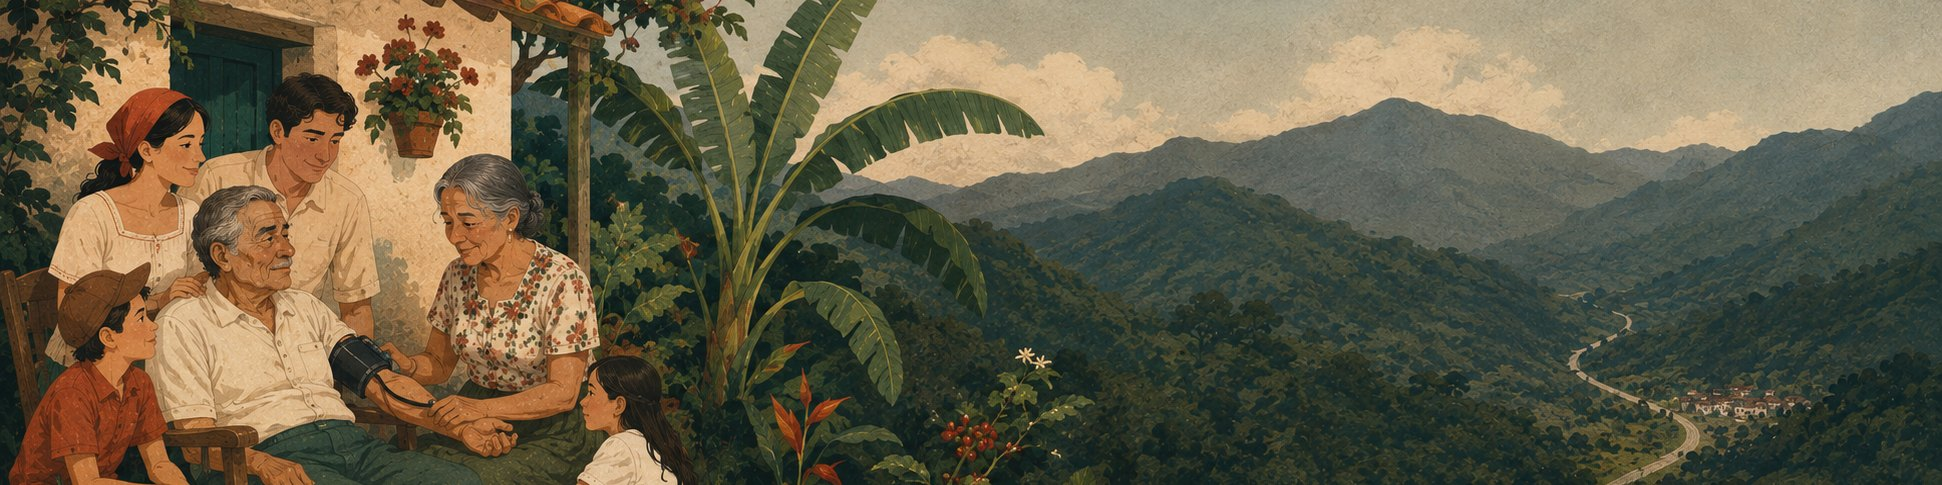
\includegraphics[width=\linewidth]{figuras/portada.jpg}
\vspace{1.1cm}

\begin{tabular}{rl}
\textcolor{muted}{Repositorio} & \url{https://github.com/cmorregof/homecare}\\
\textcolor{muted}{Bot} & \url{https://t.me/project918_homecare_bot}\\
\textcolor{muted}{Panel} & \url{https://homecare-bice-beta.vercel.app}\\
\end{tabular}

\vfill
{\small\textcolor{muted}{Documento generado el \today}}
\end{titlepage}

\pagenumbering{roman}
\tableofcontents
\newpage
\pagenumbering{arabic}

% =====================================================================
\section{Qué es CARMEN}
\markboth{Qué es CARMEN}{}

CARMEN es un sistema multiagente para el seguimiento domiciliario y el triaje
de riesgo cardio-cerebrovascular en entornos de bajos recursos. Lleva el nombre
de la enfermera de confianza del barrio: la persona a la que se le cuenta cómo
se siente uno antes que a nadie.

El sistema hace tres cosas. Recibe signos vitales tomados en casa, estima un
nivel de riesgo con un modelo entrenado y reglas clínicas duras, y avisa al
equipo de la IPS cuando ese riesgo lo amerita. Alrededor de eso hay una
conversación: CARMEN pregunta, entiende respuestas en lenguaje corriente y
responde con la voz de una abuela que sabe de esto.

\subsection*{Tres puertas de entrada}

\begin{table}[htbp]\centering
\begin{tabular}{@{}lll@{}}
\toprule
\textbf{Canal} & \textbf{Para quién} & \textbf{Estado} \\
\midrule
Bot de Telegram & Paciente en casa & En producción \\
Panel web & Paciente, IPS y administración & En producción \\
API REST (FastAPI) & Integraciones & En producción \\
\bottomrule
\end{tabular}
\caption{Formas de interactuar con el sistema.}
\end{table}

No existe una aplicación móvil nativa: el canal móvil es el bot de Telegram,
donde CARMEN ya conversa, guía la toma de signos y alerta al médico asignado.

% =====================================================================
\newpage
\section{Arquitectura}
\markboth{Arquitectura}{}

\begin{table}[htbp]\centering
\begin{tabular}{@{}ll@{}}
\toprule
\textbf{Pieza} & \textbf{Tecnología} \\
\midrule
Backend & FastAPI (Python 3.12) \\
Base de datos & Supabase (PostgreSQL con RLS) \\
Modelo de riesgo & LightGBM con explicabilidad SHAP \\
Pronóstico & CARMEN-Forecast (TinyTemporalTransformer) \\
Recuperación clínica & RAG sobre guías MINSALUD, NEWS2 y MEWS \\
Voz del agente & GPT-4o sobre un núcleo determinista \\
Frontend & Next.js 14 (App Router) y Tailwind CSS \\
Bot & python-telegram-bot \\
Despliegue & Railway (backend) y Vercel (frontend) \\
\bottomrule
\end{tabular}
\caption{Componentes del sistema.}
\end{table}

\subsection{Principios que no se negocian}

Hay cuatro decisiones estructurales que el resto del sistema da por sentadas.
Cambiarlas no es refactorizar, es construir otro producto.

\begin{enumerate}
\item \textbf{La portería de rol vive en el servidor.} El
  \texttt{middleware.ts} consulta \texttt{profiles.role} en Supabase antes de
  entregar cualquier ruta protegida. El cliente no decide qué puede ver.
\item \textbf{La sesión vive en una cookie \texttt{httpOnly}} leída en
  servidor. No hay tokens en \texttt{localStorage}.
\item \textbf{RLS es la frontera de seguridad}, no la interfaz. Una consulta
  mal hecha desde el cliente no devuelve datos ajenos porque la base lo impide.
\item \textbf{Los umbrales clínicos viven en un único sitio}, el backend
  (\texttt{risk\_levels.py} y \texttt{nurse\_agent.py}). Ninguna
  pantalla calcula un nivel de riesgo por su cuenta.
\end{enumerate}

\subsection{Endpoints principales}

\begin{table}[htbp]\centering
\begin{tabular}{@{}lp{8.6cm}@{}}
\toprule
\textbf{Ruta} & \textbf{Qué hace} \\
\midrule
\texttt{POST /agents/vital-report} & Recibe signos vitales, predice riesgo,
  guarda el reporte y dispara alerta si procede \\
\texttt{POST /agents/chat} & Conversación libre con CARMEN \\
\texttt{POST /ml/predict} & Predicción de riesgo sin efectos secundarios \\
\texttt{POST /ml/forecast} & Probabilidad de deterioro a 6, 12 y 24 horas \\
\texttt{GET /models} & Métricas de los modelos entrenados \\
\texttt{POST /telegram/webhook} & Entrada del bot \\
\texttt{GET /patients}, \texttt{/vitals}, \texttt{/alerts}, \texttt{/reports} & Lectura de entidades \\
\bottomrule
\end{tabular}
\caption{Superficie HTTP del backend.}
\end{table}

% =====================================================================
\newpage
\section{Puesta en marcha}
\markboth{Puesta en marcha}{}

\subsection{Variables de entorno}

Se declaran en \texttt{.env.example}. El script
\texttt{scripts/check\_env.py} valida que estén completas antes de desplegar.

\begin{table}[htbp]\centering
\begin{tabular}{@{}lp{7.4cm}@{}}
\toprule
\textbf{Variable} & \textbf{Para qué} \\
\midrule
\texttt{SUPABASE\_URL} & Proyecto de Supabase \\
\texttt{SUPABASE\_SERVICE\_KEY} & Clave de servicio, solo backend \\
\texttt{SUPABASE\_ANON\_KEY} & Clave pública \\
\texttt{OPENAI\_API\_KEY} & Voz de CARMEN y reporte del médico \\
\texttt{TELEGRAM\_BOT\_TOKEN} & Bot \\
\texttt{ML\_MODEL\_PATH} & Bundle de LightGBM \\
\texttt{NEXT\_PUBLIC\_SUPABASE\_URL} & Frontend: sesión y tiempo real \\
\texttt{NEXT\_PUBLIC\_SUPABASE\_ANON\_KEY} & Frontend: idem \\
\texttt{NEXT\_PUBLIC\_API\_URL} & Frontend: dónde vive el backend \\
\bottomrule
\end{tabular}
\caption{Variables imprescindibles.}
\end{table}

\textbf{Cuidado con las dos últimas del frontend.} Si
\texttt{NEXT\_PUBLIC\_SUPABASE\_URL} o su clave faltan o están mal, el panel
\emph{no falla}: sirve datos de demostración. Eso se explica en la
sección~\ref{sec:demo}.

\subsection{Backend}

\begin{lstlisting}
# Con Docker (levanta también un PostgreSQL con pgvector)
docker compose up --build

# O directamente
cd backend
pip install -r requirements.txt
uvicorn main:app --reload --port 8000
\end{lstlisting}

\subsection{Frontend}

\begin{lstlisting}
cd frontend
npm ci
npm run dev        # desarrollo, http://localhost:3000
npm run build      # produccion
npm run typecheck  # tsc --noEmit
npm run lint       # next lint
\end{lstlisting}

\subsection{Integración continua}

Dos flujos en \texttt{.github/workflows/}. \textbf{Frontend CI/CD} corre
\texttt{lint}, \texttt{build} y \texttt{typecheck}, y despliega a Vercel al
integrar en \texttt{main}. \textbf{Backend CI/CD} compila, corre la suite de
pytest, valida el entorno y construye la imagen Docker, con despliegue a
Railway.

Conviene saber que \textbf{Tailwind descarta en silencio las clases que no
reconoce}. Una clase mal escrita no rompe el \texttt{build} ni el
\texttt{typecheck}: simplemente no pinta nada. Verde en CI no equivale a
correcto en pantalla.

% =====================================================================
\newpage
\section{Los tres espacios de rol}
\markboth{Los tres espacios de rol}{}

El \texttt{middleware.ts} protege tres prefijos: \texttt{/patient},
\texttt{/ips} y \texttt{/admin}. Cualquier ruta fuera de ellos queda sin
portería, así que toda pantalla que lea o escriba datos clínicos debe vivir
bajo uno de los tres.

\begin{table}[htbp]\centering
\begin{tabular}{@{}lll@{}}
\toprule
\textbf{Rol} & \textbf{Ruta} & \textbf{Para qué} \\
\midrule
Paciente & \texttt{/patient/dashboard} & Riesgo actual, signos y tendencia \\
         & \texttt{/patient/vitals/new} & Registrar una medición \\
         & \texttt{/patient/history} & Historial paginado \\
         & \texttt{/patient/chat} & Conversación con CARMEN \\
\midrule
IPS & \texttt{/ips/dashboard} & Pacientes priorizados por riesgo \\
    & \texttt{/ips/patients} & Listado asignado \\
    & \texttt{/ips/patients/[id]} & Ficha clínica \\
    & \texttt{/ips/alerts} & Centro de alertas en tiempo real \\
    & \texttt{/ips/chat} & Consulta clínica con CARMEN \\
\midrule
Administración & \texttt{/admin/dashboard} & Métricas del sistema \\
               & \texttt{/admin/users} & Gestión de usuarios \\
               & \texttt{/admin/models} & Rendimiento de los modelos \\
               & \texttt{/admin/rag} & Documentos indexados \\
\midrule
Público & \texttt{/login}, \texttt{/register} & Acceso \\
\bottomrule
\end{tabular}
\caption{Las quince rutas del panel.}
\end{table}

\pantalla{login.jpg}{Pantalla de entrada. La ilustración de portada
acompaña a la marca; el formulario cede su sitio a tres accesos de prueba
cuando Supabase no está configurado.}{login}

\pantalla{patient.jpg}{Panel del paciente. El nivel de riesgo y su
probabilidad los decide el servidor; la pantalla solo los pinta.}{patient}

\pantalla{ips.jpg}{Panel de la IPS. Los pacientes se ordenan por gravedad y
la columna de tendencia codifica el riesgo en la altura de la barra, no solo
en el color.}{ips}

% =====================================================================
\newpage
\section{Cómo entra una medición}
\markboth{Cómo entra una medición}{}

\subsection{Por Telegram}

El paciente escribe al bot. CARMEN guía la toma paso a paso, acepta
respuestas en lenguaje corriente (\emph{noventa y siete}, \emph{sí, así es})
y valida cada dato antes de seguir. Es el camino que ya usaban los pacientes
antes de existir el formulario web.

\subsection{Por el panel web}

\pantalla{vitals-new.jpg}{Formulario de captura en
\texttt{/patient/vitals/new}.}{captura}

El formulario envía a \texttt{POST /agents/vital-report} con
\texttt{source: "web"}. Cuatro decisiones merecen explicación.

\textbf{Los rangos son los del servidor, no los del formulario.} Están
espejados del validador del servidor (\texttt{nurse\_agent.py}) y el código
lleva una
nota que prohíbe estrecharlos localmente. La razón es concreta: un formulario
más estrecho que la fisiología que vigila rechaza justo las mediciones que
importan.

\begin{table}[htbp]\centering
\begin{tabular}{@{}lrr@{}}
\toprule
\textbf{Signo} & \textbf{Mínimo} & \textbf{Máximo} \\
\midrule
Presión sistólica (mmHg) & 50 & 260 \\
Presión diastólica (mmHg) & 30 & 160 \\
Frecuencia cardíaca (lpm) & 25 & 220 \\
Frecuencia respiratoria (rpm) & 6 & 50 \\
Saturación de oxígeno (\%) & 1 & 100 \\
Temperatura (°C) & 30 & 43 \\
Glucosa (mg/dL) & 20 & 600 \\
Peso (kg) & 25 & 300 \\
Dolor, mareo y disnea & 0 & 10 \\
\bottomrule
\end{tabular}
\caption{Rangos de plausibilidad. Presión sistólica, diastólica y frecuencia
cardíaca son obligatorias; el resto es opcional.}
\end{table}

\textbf{Se envía el instante completo, no la fecha.} La columna
\texttt{recorded\_at} es \texttt{TIMESTAMPTZ} y la cadencia de monitoreo es de
seis horas: guardar solo el día perdería el orden de las tomas.

\textbf{Incluye frecuencia respiratoria y temperatura}, dos de los seis
signos que el modelo de pronóstico usa.

\textbf{No hay lógica clínica en el cliente.} El formulario no calcula
niveles ni colorea por umbral propio. El nivel, la probabilidad y el texto que
aparecen tras enviar son literalmente lo que devolvió el servidor.

\subsection{Qué hace el servidor con el dato}

\begin{enumerate}
\item Valida rangos y campos obligatorios.
\item Predice el riesgo con LightGBM, o con reglas clínicas si el modelo no
  carga.
\item Aplica \textbf{anulaciones duras}: sistólica $\geq$ 180 o $<$ 80,
  frecuencia cardíaca $>$ 130 o $<$ 40, saturación $<$ 88, glucosa $>$ 400 o
  $<$ 50. Cualquiera de ellas eleva el caso a crítico sin importar qué dijo el
  modelo.
\item Redacta el reporte clínico apoyado en las guías indexadas.
\item Notifica al médico asignado por Telegram si el riesgo lo amerita.
\end{enumerate}

% =====================================================================
\newpage
\section{El sistema visual}
\markboth{El sistema visual}{}

La identidad visual está portada del trabajo del equipo de
\texttt{salud-cardiaca-web}: colores, radios, sombras y escala tipográfica
salen de su hoja de estilos. Se tomaron valores y estructura de marcado;
ninguna línea de su código entró al repositorio.

\subsection{Una desviación deliberada}

En el original, el color primario y el de peligro son prácticamente el mismo
rojo. Allí no importa porque su producto no tiene niveles de riesgo. Aquí el
rojo \emph{significa} crítico, así que el primario se desplazó al azul y el
rojo quedó reservado por completo para gravedad.

\begin{table}[htbp]\centering
\begin{tabular}{@{}llp{5.6cm}@{}}
\toprule
\textbf{Token} & \textbf{Valor} & \textbf{Uso} \\
\midrule
\texttt{brand} & \textcolor{brand}{\rule{2.4ex}{1.6ex}} \texttt{\#1976D2} & Botón primario, enlaces, activo \\
\texttt{brand.dark} & \textcolor{brandDark}{\rule{2.4ex}{1.6ex}} \texttt{\#0D47A1} & Degradados y estados \\
\texttt{risk.low} & \textcolor{riesgoBajo}{\rule{2.4ex}{1.6ex}} \texttt{\#2E7D32} & Riesgo bajo \\
\texttt{risk.moderate} & \textcolor{riesgoModerado}{\rule{2.4ex}{1.6ex}} \texttt{\#ED6C02} & Riesgo moderado \\
\texttt{risk.high} & \textcolor{riesgoAlto}{\rule{2.4ex}{1.6ex}} \texttt{\#C62828} & Riesgo alto \\
\texttt{risk.critical} & \textcolor{riesgoCritico}{\rule{2.4ex}{1.6ex}} \texttt{\#9A0007} & Riesgo crítico \\
\bottomrule
\end{tabular}
\caption{Colores con significado. Radios 6/10/16/24\,px, tres sombras y base
tipográfica de 14\,px completan el sistema.}
\end{table}

\subsection{Por qué los niveles no se distinguen solo por color}

\texttt{risk.high} y \texttt{risk.critical} son dos rojos oscuros. El
contraste entre ellos es de \textbf{1{,}57:1}, y con deuteranopía es aún
menor. Quien no separe esos dos tonos no podría distinguir un paciente de
riesgo alto de uno crítico: la distinción más consecuente del producto.

Por eso cada nivel difiere en cuatro canales a la vez.

\begin{table}[htbp]\centering
\begin{tabular}{@{}lllll@{}}
\toprule
\textbf{Nivel} & \textbf{Relleno} & \textbf{Texto} & \textbf{Peso} & \textbf{Contraste} \\
\midrule
Bajo & tinte al 8\,\% & verde & 600 & 4{,}63:1 \\
Moderado & sólido & oscuro & 600 & 4{,}72:1 \\
Alto & contorno de 2\,px & rojo & 700 & 5{,}62:1 \\
Crítico & sólido & blanco & 800 & 8{,}83:1 \\
\bottomrule
\end{tabular}
\caption{Los cuatro niveles superan WCAG AA, medido sobre el DOM renderizado.
Cada uno lleva además un icono distinto.}
\end{table}

Leídos en escala de grises, los rellenos van de claro a muy oscuro y la
polaridad texto/relleno se invierte dos veces, de modo que el orden sobrevive
sin ninguna información de tono. El par alto/crítico, que el color no puede
separar, queda a \textbf{8{,}83:1} como tratamientos.

\pantalla{tiers-normal.jpg}{Los cuatro niveles en visión normal.}{tiersnormal}

\pantalla{tiers-deut.jpg}{Los mismos, simulando deuteranopía. Los distintivos
siguen siendo distinguibles; la columna de tendencia también, porque codifica
la gravedad en la altura de la barra.}{tiersdeut}

% =====================================================================
\newpage
\section{Modo demostración}\label{sec:demo}
\markboth{Modo demostración}{}

El panel puede servir datos inventados en dos situaciones distintas, y solo
una tiene que ver con la configuración.

\textbf{Primera: Supabase no está configurado.} Todas las lecturas
retroceden a \texttt{lib/mock-data.ts}. Una variable de entorno mal puesta en
producción deja el producto entero en este estado.

\textbf{Segunda, y más peligrosa: Supabase está configurado y sano, y aun así
hay datos inventados.} El listado de pacientes de la IPS, las alertas de cada
ficha y todo el panel de administración salen de los mocks sin importar la
configuración.

Un aviso que solo mirara la configuración habría permanecido oculto
justamente en el segundo caso. Por eso el banner nombra \emph{qué} conjuntos
son ficticios, y se acompaña de un \texttt{console.warn} en cada una de las
ocho ramas que sirven mocks.

\pantalla{alerts.jpg}{El banner de datos de demostración. Evita
deliberadamente los tonos de peligro y advertencia: esos significan «este
paciente está en riesgo», y este significa «nada de esto es un
paciente».}{demo}

% =====================================================================
\newpage
\section{Base de datos}
\markboth{Base de datos}{}

\begin{table}[htbp]\centering
\begin{tabular}{@{}lp{8.2cm}@{}}
\toprule
\textbf{Tabla} & \textbf{Contenido} \\
\midrule
\texttt{profiles} & Persona y rol; enlaza con \texttt{auth.users} \\
\texttt{ips} & Instituciones prestadoras \\
\texttt{patient\_clinical\_info} & Antecedentes y línea base \\
\texttt{vital\_signs} & Cada toma, con su origen y su instante \\
\texttt{risk\_predictions} & Nivel, probabilidad y factores \\
\texttt{clinical\_reports} & Interpretación y recomendaciones \\
\texttt{alerts} & Avisos al equipo clínico \\
\texttt{rag\_documents} & Guías clínicas indexadas \\
\bottomrule
\end{tabular}
\caption{Esquema principal, en \texttt{backend/db/schemas.sql}.}
\end{table}

\subsection{Migración propuesta y no aplicada}

\texttt{backend/db/migrations/20260902\_add\_demographics.sql} añade a
\texttt{profiles} siete columnas de contexto colombiano: EPS, grupo étnico
según categorías DANE, clasificación de insuficiencia cardiaca A--D, fecha de
nacimiento, sexo biológico, departamento y ciudad. Es idempotente y está
verificada aplicándola dos veces contra un PostgreSQL desechable.

\textbf{Antes de aplicarla hay que resolver un solapamiento.}
\texttt{patient\_clinical\_info} ya guarda \texttt{age} y \texttt{gender}, que
se solapan con \texttt{birth\_date} y \texttt{biological\_sex}. Aplicarla tal
cual deja dos fuentes para el mismo hecho, libres de divergir. Y una edad
almacenada es correcta el día que se escribe y falsa a partir del siguiente
cumpleaños. La migración solo añade columnas: resolver el solapamiento es una
decisión aparte.

% =====================================================================
\newpage
\section{Decisiones abiertas}
\markboth{Decisiones abiertas}{}

\begin{enumerate}
\item \textbf{El solapamiento demográfico.} Poblar \texttt{birth\_date},
  deprecar \texttt{age} y calcular la edad al consultar, o mantener las dos
  fuentes conscientemente.
\item \textbf{Aplicación móvil nativa.} Hoy el canal móvil es Telegram. Una
  app nativa no lo extiende, lo duplica; habría que decidir si conviven.
\item \textbf{Los datos que el panel muestra y la base no tiene.} El nombre
  del usuario en la barra lateral y los umbrales de la gráfica de tendencia
  están preparados pero sin cablear, a la espera de que alguien los sirva.
\item \textbf{El buscador de pacientes} de la IPS es decorativo: no está
  conectado a ninguna consulta.
\end{enumerate}

% =====================================================================
\appendix
\newpage
\section{Cómo compilar este documento}
\markboth{Cómo compilar este documento}{}

\begin{lstlisting}
cd docs/manual
pdflatex manual.tex
pdflatex manual.tex   # la segunda pasada resuelve el indice
\end{lstlisting}

Requiere una instalación estándar de TeX Live. En Debian o Ubuntu:

\begin{lstlisting}
sudo apt-get install texlive-latex-base texlive-latex-recommended \
                     texlive-fonts-recommended texlive-lang-spanish lmodern
\end{lstlisting}

El documento usa solo \texttt{graphicx}, \texttt{xcolor}, \texttt{geometry},
\texttt{hyperref}, \texttt{booktabs}, \texttt{fancyhdr}, \texttt{listings},
\texttt{babel} y \texttt{lmodern}, todos incluidos en esos paquetes. No
requiere \texttt{titlesec}, \texttt{tcolorbox} ni \texttt{enumitem}. Las figuras están en
\texttt{figuras/} y son capturas de la aplicación en ejecución.

\end{document}
